\begin{frame}
    \frametitle{Restbudget}
    \begin{itemize}
        \item[] Menge verbleibender Emissionen bis zur Erreichung bestimmter Temperaturererhöhungen
    \end{itemize}
    
	\begin{figure}
		\centering
		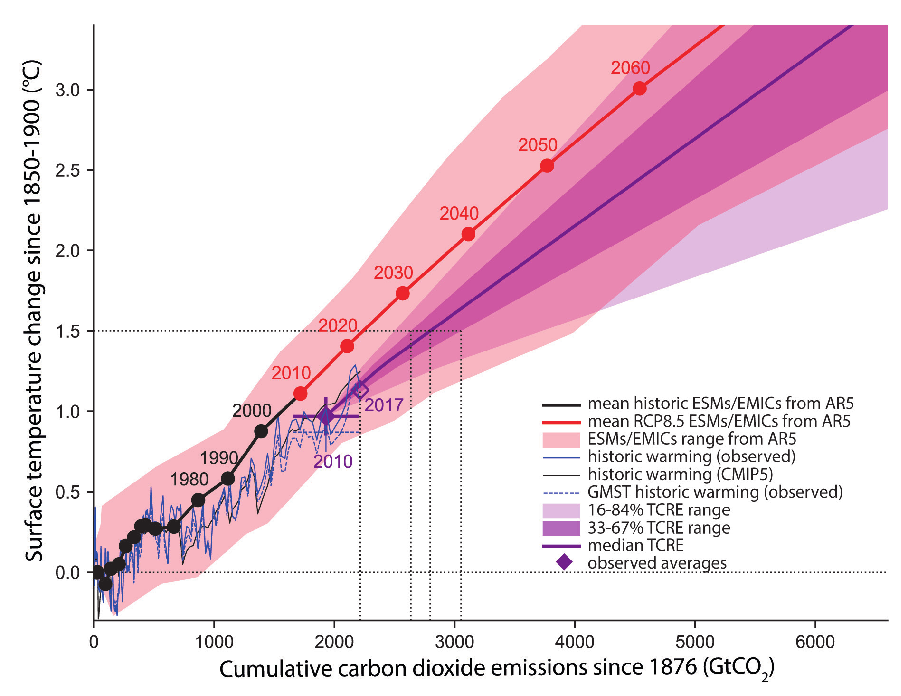
\includegraphics[height=.8\textheight]{bilder/cumulative_co2.pdf}
		\caption{Globale Oberflächentemperatur gegen kumulative CO$_2$-Emissionen.}
	\end{figure}
\end{frame}

\begin{frame}
	\frametitle{CO$_2$ Restbudget für Erwärmung um 1,5°C}

    \begin{itemize}
        \item[] 420 GtCO$_2$ zur Einhaltung mit 66\% Warscheinlichkeit
        \item[] 580 GtCO$_2$ zur Einhaltung mit 50\% Warscheinlichkeit
        \item[] Reduktion um 100 GtCO$_2$ bei Berücksichtigung von Erdsystem-Rückkopplungen wie Auftauen von Permafrostböden
    \end{itemize}

	\note{
		\begin{itemize}
			\item[] Restbudgets einerseits aus Erwärmung im Vergleich zu 1861-1880 auf Basis des RCP8.5 Szenarios
            \item[] Andererseits \"from a set of available pathways that were assessed to have a >50\% probability to exceed 1.5°C by mid-century, and return to 1.5°C or below in 2100 with greater than 66\% probability\"
            \item[] Weitere Studien, die teilweise nur CO$_2$ berücksichtigen
            \item[] Seit dem AR5 Report 2014 viele weitere Veröffentlichungen, die berücksichtigt werden
            \item[] Viele Unsicherheiten auf die berechneten Restbudgets wie Unterschiede in Szenarien zur Entwicklung von nicht-CO$_2$ Emissionen oder die Unsicherheit auf die historische Temperatur von 1850-1900

		\end{itemize}
	}
\end{frame}


